\section{Modeling Methods and assumptions}
In addition to the diagnostic inputs, there are various details of how the model is put together that serves to inform the discussion of the results. These topics include data selection and ensembling, equilibrium reconstruction, and similar modeling considerations, as well as the particulars of the initial conditions and boundary conditions. 
%%% The above statement doesn't really say much. Hopefully you are providing the right level of detail throughout all of your writing :) -- MDN
%----
%Noted, removed statement. -X

\subsection{Shot selection criteria and ensembling of diagnostic inputs}

The modeling work revolves around the ion transport in well-behaved PPCD periods. Data from the PPCD periods included in the ensemble are selected according to the following criteria:
\begin{itemize}
\item periods with little or no burst activity as determined from magnetic fluctuations and poloidal gap voltage measurements; 
\item early onset of enhanced electron confinement (12~msec or earlier) determined by a systematic rise in soft x-ray emission;
\item density and current approximately in range of the rest of the shots used ($n \approx 0.7 \times 10^{19} /m^3$ and $I_p \approx 480 - 500kA $) at their peak during the PPCD period;
% Specify the density and current ranges used to select shots. Is the initial density 5 \times 10^18 m^{-3} \pm 10^18 for instance? 
%----
%Clarified -X
\item reliable operation of the interferometer and Thomson Scattering diagnostics.
\end{itemize}
The ensemble of ion temperature measurements are drawn from CHERS data from a larger set of shots. The spectrometer gives single-point measurements and building up an ensemble of data to reconstruct the evolution of the ion temperature profiles requires many more shots. These shots are chosen by the same criteria as listed above, but the ensemble includes days where the FIR interferometer and Thomson Scattering diagnostics are unavailable.


\subsection{Equilibrium reconstruction through MSTfit}\label{sec:MSTfit}

% To which code are you referring here? It's not quite clear in the context of the Chapter.

% You also need an introduction to what is entailed in an "equilibrium reconstruction," and what is MSTfit. You are assuming that all of the relevant ion heat transport processes operate on the radial transport time scale. Transport along field lines (and within flux surfaces) operate by ions streaming at the thermal speed along a field line. This process is considered fast enough to equilibrate the ion distribution function within a flux surface. The question then becomes, what is the geometry of the magnetic flux surfaces and what is the temperature and density on each of the nested flux surfaces. Since the ions are equilibrated quickly within flux surfaces, the only remaining pressure gradient is in the radial direction. Write down the radial pressure balance equation, assume that the magnetic field and current density can be written in terms of flux coordinates, and then you have the Grad-Shafranov equation. MSTfit solves the Grad-Shafranov equation constrained by the available data from the diagnostics described above. Your ion heat transport model makes use of iterative solutions of the Grad-Shafranov equation to determine changes in the ion heating and cooling mechanisms over transport time scales.
%----
%Noted, Currently correcting. -Xing
As discussed in the previous chapter, the 1-D model relies on the fact that the transport within flux surfaces are well equilibrated on the time scale of interest, and relatively well formed compared to standard RFP plasmas. Plasma parameters, with exceptions of neutral calculations, are thus treated as flux surface quantities in a cylindrical approximation. The determination of the quasi-equilibrium magnetic geometry is done by a process referred to as equilibrium reconstruction through the MSTfit code. Given a set of magnetic, density and temperature measurements, MSTfit uses a non-linear solver to find the best fit 2-D solution to the Grad Shafranov equation:
\begin{align}
    J_(\phi) &= \frac{2\pi F F'}{\mu_0 R} + 2\pi Rp'
\end{align}
where $F = RB_{\phi}$ and $p$ is the pressure, assumed to be isotropic. The reconstruction code further assumes a symmetric plasma, which is well suited for PPCD. In doing so, the FIR measurements of density and internal magnetic field, as well as Thomson Scattering measurements of $T_e$ are used as part of the constrain data. The details of how this is achieved can be found in J. Anderson's thesis \cite{Anderson2001} and paper \cite{Anderson2004}. The result of this process is a set of flux surfaces with associated temperature and density, as well as associated magnetic field.  Because of this, the electron density measurement is not of an independent inversion of line integrated measurement, but a part of the non linear fit; same applies to magnetic field and electron temperature. 

The transport model takes advantage of this existing code base by reading these information as input. To cover the entire period of interest, as series of MSTfit reconstructions are produced. In order to conduct ensemble analysis, the input diagnostic data is ensembled across the list of shots and then the series of reconstruction is produced for the code. Each of theses fits corresponds to what I term time blocks, the larger time scale of model propagation usedfor the input of plasma parameters. The actual propagation of the model occurs over two time scales. I distinguish the two with the names of time \textit{blocks} (the larger, slower steps) and time \textit{steps} (the smaller, faster propagation steps). 


\subsection{Time blocks and time steps}\label{sec:time_blocks_and_steps}

The model is associated with two pertinent time step sizes. The model code is flexible in what size these steps sizes are for a particular analysis, but for the analysis in this work they are set at ~ 0.5ms and 1$\mu s$ respectively. The slower timescale already mentioned above is the one use for updating the magnetic equilibrium and associated input plasma parameters via MSTfit as well as neutral calculations via DEGAS2 simulations. The PPCD quasi-equilibrium being considered are very stable and slow evolving. The electron temperature confinement time has been previously evaluated to be ~10ms\cite{Chapman2001} and ion confinement is expected to be similar or better, where as the transient nature of PPCD causes the $T_e$ to approximately double in 10ms, setting the effective time scale. Fast dynamics such as turbulence are only relevant to the physics scope of the model in time averaged sense. Hence the ~0.5ms update timescale is sufficient to capture the relevant changes in plasma parameter. Reduction of time block size would involves trades offs with resource requirements, such as needing faster TS data collections rate and thus less overall coverage, as well as more DEGAS2 simulations that significantly impact model run time. As the results in chapter \ref{ch:results} bears out, the power terms being considered for the model, as well as measured $T_i$ also evolves slowly compared to the time block size.

The model calculations are done at a faster timescale that I call time steps. This is set at $1\mu s$ in consideration for numerical error in finite time step propagation. As mentioned in section \ref{sec:transport_summary}, the mathematical core of the model is an numerical integration in time. A rectangle-rule integration is used to simplify the various power term calculations, but it has a relatively high numerical error. The error bound by rectangle-rule integration has an upper bound of 
\begin{align}
    \text{Error} &\leq \sum_{i = 0}^{N} \frac{f'(t_i)\Delta t^2}{2} \leq \frac{N}{2}\text{Max}(f')\Delta t^2 = \text{Error}^*
\end{align}
where t refers to time. With a setting of $\Delta t = 1\mu s$, the percentage error bound,
\begin{align}
    \text{Error}^*_P = \frac{\text{Error}^*(\int f(t))}{\int f(t)}
\end{align}
where $f(t)$ refers to the $\partialt E_{\text{thermal}}$ function as defined in section \ref{sec:transport_summary}, comes to $\approx 0.1\%$. This is due to the low rate of change in the energy function as compared to step size. Of course the verification is performed after the analysis, but conceivably the time step does not need to be so small. 




%The most basic is what I term a time \textit{step}, this is set arbitrarily %%% I would caution against saying that the shortest time step you chose was arbitrary. I think that this time step serves as an interpolation 
%at 1$\mu$s which is much faster than the time scale of the physics under investigation. The transport model terms themselves are calculated (or in the case of the neutral modeling discussed in the next sections, interpolated) per time step, and can smoothly evolve in time. The fine timescale is sufficient to minimize the error and instability associate with finite element (time, in this case) approximation.

%%% Each of these reasons are really only superficial to your analysis. Indeed, you are limited by the rate at which Thomson scattering data are acquired and the frequency with which you perform equilibrium reconstructions. The plasma doesn't care about these limitations, however. The more fundamental question is how quickly does the magnetic equilibrium and the temperature and density profiles evolve? There is already existing work showing that the electron energy confinement time in standard RFP plasmas is about 1 msec and in PPCD plasmas is about 10 msec. Since we expect the ions to be better confined than the electrons, we expect the ion heat transort term to change no faster than the electron transport. Therefore transport losses should be adequatly modeled using a time block of 0.5 msec. Each of the source and sink terms in the ion energy balance equation are expected to evolve on a timescale no faster than this as well since we are eliminating data from any discharges that have burst activity which introduces rapid heating on a shorter timescale (about 100 microseconds). After justifying how fast to expect the different source and sink terms to vary, you can then justify the data acquisition rate for the different diagnostic measurements used for the ion heat transport model and the time step over which to evolve the model.

%The first is that MSTfit, in it's standard configuration, takes data inputs from a 0.25ms window for it's equilibrium reconstruction. Since the input data is an ensemble of shots, it is conceivable to run MSTfit calculations with a smaller window more often, it is not a particularly urgent concern as the model is aimed to capture faster time scale physics, and the PPCD plasmas themselves do not contain physics that would show themselves in a somewhat faster tempo of equilibrium reconstruction. The more important constraint on the time block size is the data-rate of the Thomson Scattering diagnostic at 2kHz. $T_e$ is an important input that helps MSTfit determine the pressure term in equilibrium reconstruction. If the TS measurement is unavailable, MSTfit uses a mock $T_e$ profile based on plasma current, but it is insufficient for high current PPCD plasmas. If a mixture of MSTfit reconstructions, some with and some without TS measurement of $T_e$ is used for the model, then an unacceptable amount of 'wobble' in the reconstructed flux surfaces would occur as the model goes from a TS based reconstruction to a TS free reconstruction. Similarly, as the interpretation of both the FIR interferometry and polarimetry measurement is aided by the flux surface reconstruction, it does not make sense to try to incorporate those at a higher frequency either. Again, the result of simple inversions of line integrated FIR measurements is sufficiently different from those aided by equilibrium reconstruction that it would detract from the model. Finally, the DEGAS2 neutral simulation (section \ref{sec:DEGAS2}) also depends on the $T_e$ profile significantly. Thus, then only diagnostic that meaningfully independent of TS's timescale is the charge exchange measurement of $T_i$, which serves as a comparison to the model's predictions. However, despite the fact that diagnostic inputs are made available to the model via MSTfit every time block, they are spline interpolated onto the smaller time steps to avoid sudden jumps in profiles.

\subsection{Monte-Carlo neutral simulation through DEGAS2}\label{sec:DEGAS2}

As mentioned in section \ref{sec:dalpha_array}, the neutral dynamics are more difficult to ascertain than the physics of the $\dal$ emissions would suggest. This is because the neutral density drops very significantly towards the core of the plasma such that it contributes a negligible portion of the $\dal$ emission observed. Simple inversions are not able to determine the core neutral density effectively, especially for PPCD plasmas where the neutral density and resulting $\dal$ emission levels are significantly lower than in standard plasmas. At the same time, although the low neutral density results in insignificant light emission, this does not mean that it can be ignored. Even though the neutral density is a tiny fraction of $n_e$ ($~1\times 10^{-4} to 1\times 10^{-5}$), the charge exchange reaction of this low density gas with ions in the hot core is an important heat transport channel. To asses the neutral dynamics and how it effects the ion thermal transport, a Monte-Carlo simulation is needed. A Monte Carlo neutral simulation initializes a large number of test particles and tracks their behavior though the plasma in physics-based probabilistic calculations. Net characteristics of the neutral population can then be tallied though the net behavior of all the test particles. Monte Carlo simulation are the standard for neutral dynamic calculations since the neutral mean free path is too large to justify a fluid approximation. Additionally, the neutral population does not necessarily satisfy the same symmetries as the charged particle populations (poloidally-symmetric flux surfaces for example). Unfortunately, Monte Carlo simulations are costly in terms of computing power, and are the calculations that set the pace for the model calculation time. 

The Monte Carlo simulation code used for this work is DEGAS2 developed at PPPL\cite{Stotler}. It is a 2-D simulation that takes 2-D $T$ and $n$ profiles as input and tracks and tallies charge exchange, ionization, recombination, and molecular disassociation reactions, as well as associated particle and heat flow of test particles. For this work, it is setup with 3 source terms at the edge of the plasma (details on their geometry are presented in section \ref{sec:neutral_source_geometry}) and synthetic $\dal$ emission detectors to predict measurements made by the $\dal$ array on MST. The detailed physics of sputtering, recycling, and sublimation underlying the neutral source from the different wall and limiter materials are outside of the scope of this work. The simulations are run such that neutral molecules enter the plasma at a defined rate and geometrical extent, they evolve into different charged and neutral species according to the appropriate rate coefficients, the neutral and charged particle populations are tallied, and the radiance observed by the synthetic detectors is predicted. The neutral source rates are used by the broader model as fitting parameters used to achieve a fit between the predicted $\dal$ emission and the observed data. Conveniently, DEGAS2 tallies quantities of interest such as charge exchange ion loss (a neutral source), particle source rates, and energy associated with ionization directly, which means the model takes the 2-D output of these value and incorporates them via flux surface averaging. While the neutral profiles are \textit{not} flux surface quantities, the ion population travelling around the flux surface will experience the averaged effects from the neutrals, justifying the  assumption of toroidal symmetry.

DEGAS2 simulations are run for each time block (defined in the section previous) as a compromise between both due to  it's computational cost, as well as the availability of $T_e$ measurements, a very important input parameter. This arrangement has one problem, however, and that is model self-consistency. To run DEGAS2 simulations, the $T_i$ profile is needed, but for the ion heat transport model to calculate $T_i$, it needs the outputs from the DEGAS2 simulation. To alleviate this issue, the predictor and corrector method is used.

\subsection{Pseudo-self-consistency, and predictor and corrector methods}\label{sec:predictor_and_corrector}

In addition to the problem of self consistency, it would be advantageous to take into account the time variation of the neutral density profile $n_0$ and source and sink terms (like $P_{CX}$) that vary during a time block rather than modeling their values as suddenly jumping at time block boundaries. This is a concern for adequate physical accuracy both for the direct interactions between the deuterium ions and neutrals and also for the impurity charge state ratio calculations which depend on $n_0$. The impurity charge state affects density and pinch flow calculation which in turns impacts the heating terms, all of which are calculated on a time step basis. A sudden jump in the modeled neutral density profile causes unrealistic time variation of these terms at the time block boundaries. Hence then need to interpolate the power terms for each time step within a time block.

To address these issues the code uses a simple predictor-corrector implementation to propagate transport terms. This method uses the previous time point information as an approximation to 'predict' the following time step, and then uses the 'prediction' to redo part of the calculations and thus correct the values. In general, the predictor corrector method, when applied to explicit methods, can be understood mathematically as the following:

% Why not just write down the predictor-corrector equations for T_i rather than introducing the dummy variable y? Also, I think that this method is called the Euler-Trapezoidal method as you've written it. If the equation for the time derivative of y depended on spatial derivatives of y then it would be called the Crank-Nicolson method. You should note that it is a second-order-accurate numerical method. This should help in determining how short a time block should be.
%--------------
%TO MARK: see below for additions and details on predictor-corrector implementation. I feels like the two time scales bars it from being Euler-Trapezoidal or C-N as the time step propagation is itself just simple Euler. The explanation is hopefully clear, but the notation may be confusing, especially that i and e denotes species. Let me know if it is clear to you. -X
\begin{align}
    y^*(t_{i+1}) &= \Delta t\frac{\partial y}{\partial t}(t_i, y(t_i)) + y(t_i)\\
    y(t_{i+1}) &= \frac{\Delta t}{2} \left(\frac{\partial y}{\partial t}(t_i, y(t_i)) + \frac{\partial y}{\partial t}(t_{i+1}, y^*(t_{i+1})) \right) + y(t_i)
\end{align}
where $\Delta t$ is the time step size, $\frac{\partial y}{\partial t}$ is a known function, and the asterisk denotes estimation. For the purpose of my model, y would represent the $T_i$. The particular implementation with in the model is somewhat convoluted as the model has two time scales and the predictor corrector calculations are not applied to the fundamental stepsize of the model but to the time blocks. We define j as the time step index, and J as the time block index, and further, use the notation that $j_{J}$ represents the j index such that $t_{j_{J} = t_{J}}$ (\textit{i.e.} the time point represented by time step if index $j_{J}$ is the same as the time block of index $J$). Due to the ratio between the time step and time block size, $j_{J+1} = j+500$ and $j_0 = 0$. To simplify the explanation, the other (non charge exchange) power terms which are calculated for each step and not block and do not have self consistency issue introduced by the two time scales, are grouped together in notation as $P_{\text{other}}$ . In order to propagate the model from index $j_J$ to index $j_{J+1}$ (\textit{i.e.} a time block), first the charge exchange term is calculated at the beginning step:

\begin{align}
    P_{\text{CX},{j_J}} = \text{DEGAS2}(n_{i,j_J},T_{i,j_J}, n_{e,j_J}, T_{e,j_J})
\end{align}
Then the model is propagated assuming that $P_{\text{CX}}$ stays constant between index $j_J$ to index $j_{J+1}$ (\textit{i.e. }$ = P_{\text{CX}, j_J}$), because the $P_{\text{CX}, j_{J+1}}$ cannot be calculated with known information. With that, we can 'predict' $T^*_{i,j_{J+1}}$ with:
\begin{align}
    E^*_{j+1} & = \frac{3}{2}n_{i,j_1}kT_{i,j+1}^*\\
    & = P_{\text{other}, j} + P_{\text{CX}, j_J}\\
    \text{for } &j_J \leq j \leq j_{J+1}
\end{align}
with the predictor's result for $T*_{i, j_{J+1}}$, $P_{\text{CX}, j_{J+1}}$ can be calculated via DEGAS:
\begin{align}
    P_{\text{CX},{j_{J+1}}} = \text{DEGAS2}(n_{i,j_{J+1}},T*_{i,j_{J+1}}, n_{e,j_{J+1}}, T_{e,j_{J+1}})\label{eqn:P_cx_pred}
\end{align}
note that with the exception of $T_i$, the other values are diagnostic inputs and are known quantities in the context of the model and thus are not 'predicted' or 'corrected'. This also applies to $P_{\text{other}}$. Now with $P_{\text{CX}, j_{J+1}}$ calculated, next step is to prepare the 'corrector' by splining $P_{\text{CX}, j}$ for the block:
\begin{align}
    P_{\text{CX}, j} &= \text{linear interpolation}(P_{\text{CX},{j_J}}, P_{\text{CX}, j_{J+1}}, (j_{J+1} - j_J) )\\
    &= P_{\text{CX},{j_J}} + (j - j_J)(\frac{P_{\text{CX}, j_{J+1}} - P_{\text{CX},{j_J}}}{j_{J+1} - j_J})
\end{align}
with this calculated, the model propagate the steps from $j_J$ to $_{J+1}$ again for a second pass, with the splined $P_{\text{CX}}$:
\begin{align}
    E_{j+1} & = P_{\text{other}, j} + P_{\text{CX}, j}\\
    \text{for } &j_J \leq j \leq j_{J+1}
\end{align}
Where upon the block is complete and the code moves on to the next block. Further, $P_{\text{CX},{j_{J+1}}}$ has already been calculated (in equation \ref{eqn:P_cx_pred}) and can be used to start the next block. By taking this expedience, DEGAS2 is only ever run with $T_i^*$ (the 'predicted' temperature) as the input, and in theory, additional accuracy could in theory be gained by rerunning DEGAS2 after the $T_i$ calculations are redone, and circle around the 'corrector' loop again. However, this only very marginally improves the calculation as $T_i$ changes very slowly even compared to time block size, and DEGAS2 calculations are generally more sensitive to $T_e$, which is an external input to the model and does not suffer from the same prediction issues. The primary aim of applying this method is to better approximate the $P_\text{CX}$ and $\partialt n_i$ terms which are important for the model results presented in chapter \ref{ch:results}.
% This paragraph would be more readable if the predictor-corrector equation you actually use for T_i would be written above including the dependencies on n_0, P_CX, n_0^*, P_CX^*, and T_i^*.
%----
%TO MARK: See above elaboration on what the code is doing. -X
\subsection{Other considerations}

The model evolves the ion temperature according to the physics described, but to do that it is initialized with $T_i$ from CHERS measurement. However the CHERS measurement chords needs to be interpolated for use on the finer radial grid of the model. 
% You should write out the analytical form for the "alpha model" and perhaps show a plot of the fitted Ti profile for both an alpha model and a spline interpolation.
%----
%I noted the analytical form. The plot is in the works. -AX
A simple profile function for plasma quantities is the 'alpha model':
\begin{align}
    T(\rho) &= T_0(1 - \rho^\alpha)^\beta + T_{\text{edge}}
\end{align}
where $\alpha$ and $\beta$ are fitting parameters. However, it does not fit the measured $T_i$ profile well (see figure \ref{fig:init_ti}). Instead, a free-knot-spline fit is used. Additional constraints are included to make the initial profile more physical. 
\begin{figure}
	\centering
	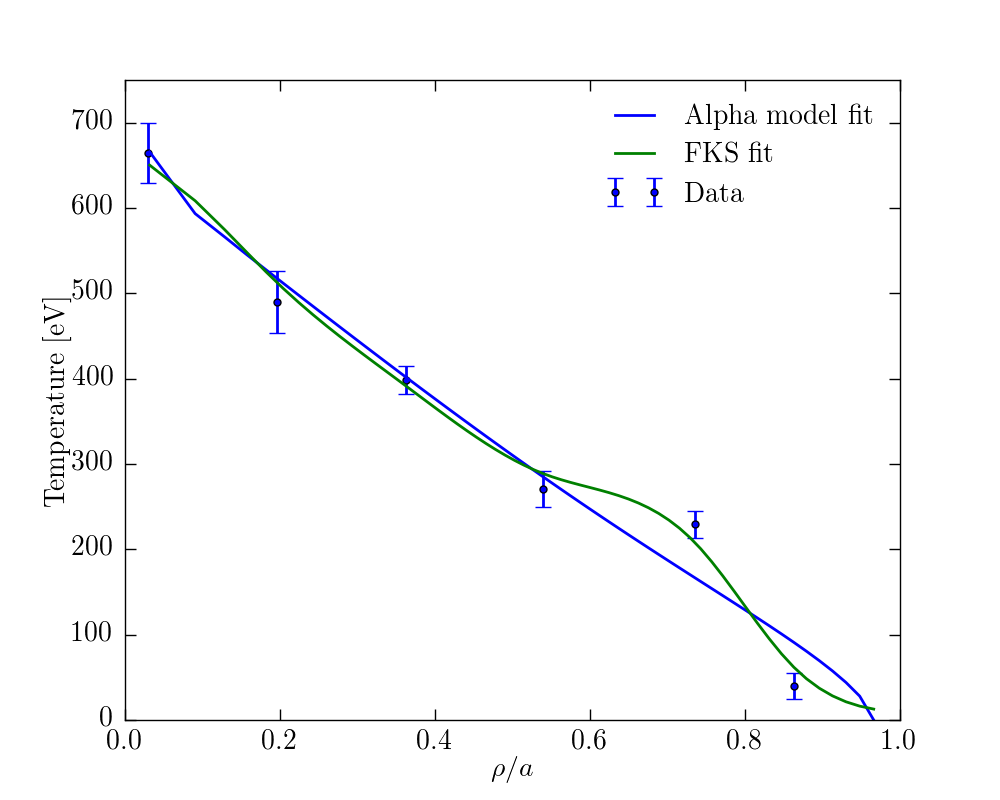
\includegraphics[width = 1.\linewidth]{./implementation/init_ti.png}
	\caption{$T_i$ initial condition and fit.}\label{fig:init_ti}
\end{figure}
% Are you creating this mirrored data in order to provide a Neumann boundary condition of zero derivative at the boundaries?
%----
%TO MARK: yes, I clarified below.
First, the data being fit are mirrored at $\rho_v < 0$ and $\rho_v > a$. This is done to impose Neumann boundary condition, which in turns is important to prevent the edge $T_i$ fit returning a negative region, and is further needed to make sure the very core point (inside the core most measurement) do not get fit to a very high temperature with a gradient. Further, two additional data points added to the CHERS measurements, one is the boundary condition of $T_i(a) = 10eV$, a standard approximation, and the other is the passive IDS measurement of the C-III (C$^{2+}$) emission line in 500kA PPCD plasmas. There are some uncertainty in the location that it corresponds to, and for the purpose of the model this data point is located at $\rho_v = 0.46$, as determined from collisional-radiative modeling of similar plasmas\cite{Nishizawa2018,Barbui2014}. These points are added to the CHERS measurement to arrive at the initial condition because the CHERS measurements by themselves do not adequately sample the ion temperature gradient at the edge.

The boundary condition of the model is largely inherited from the MSTfit reconstruction code \cite{Anderson2001} as it pertains to the input. It is useful to point out that $T_i$ at the edge most location is held constant, and the thermal energy transported to this point is considered lost from the plasma. This is necessary as the MSTfit's boundary condition imposes $n = 0$ at this point, and a temperature cannot be realistically be applied. Similarly, in calculating radial derivatives, the last radial point is ignored and the derivative extrapolated.

Further, quasi-neutrality is imposed on the model. This is to be expected, but it does broach the subject of the role of the impurities in the model. The model does not actively model impurity transport or charge-state evolution; this would be a large extension of the scope of the majority heat transport modelling. However, they are not ignored either. As will be discussed in greater detail in section \ref{sec:eb_pinch}, the radial particle velocity is needed for calculating the flow related terms, and determining the origin of the core density rise. This is calculated by using the particle continuity equation, which in turns depends on the source term and the density change. However, only the electron density is available through measurement, and as the impurities also provide an electron source through ionization, they're effect on the particle continuity equation must be determined. As such, the impurity levels (including carbon, oxygen, boron, and aluminum) are taken from M. Nornberg's work \cite{Nornberg2018}, and added to the model as constant densities with evolving charge state balance. The quasi-neutrality calculation thus includes the impurity contribution, though it is found that their contribution to $\partialt n_e$ is not especially significant in explaining the observed core density increase during PPCD (see section \ref{sec:eb_pinch}).

%\subsection{Basic plasma assumptions}

%\subsection{Role of impurities}
